\chapter{Background}
\label{ch:background}
%%%%%%%%%%%%%%%%%%%
% - description of foundational knowledge required to understand the thesis
%%%%%%%%%%%%%%%%%%%

This chapter explains the fundamental topics required to understand this thesis.

\section{Semantic Web Topics}
The following topics come from the research area of Semantic Web.
Since this thesis focuses mostly on the implementation and deployment of the Basilisk framework, these topics are mostly introduced to give a basic understanding of the context in which the Basilisk framework is used.

\subsection{Knowledge Graphs} 
\label{sec:knowledge_graphs}
Knowledge Graphs are graphs intended to represent knowledge of the real world or smaller scenarios.
The knowledge stored in Knowledge Graphs is modeled in a graph-based structure. 
Nodes represent entities which are connected by various types of relations, represented by labeled edges in the graph.
This has the benefit to represent complex relations between different nodes and edges\cite{hoganKnowledgeGraphs2021}.

The simplest knowledge graph consists of three elements.
The subject entity, the object entity and the labeled edge between them describing their relation.
This atomic data entity is called triple.
In figure \ref{fig:example-knowledge-graph} a simple example of a knowledge graph is shown.

\begin{figure}[tbph]
	\centering
	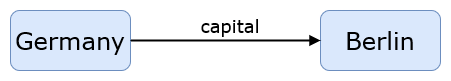
\includegraphics[width=0.4\textwidth]{figures/knowledge-graph-diagram}
	\caption{Simple Knowledge Graph}
	\label{fig:example-knowledge-graph}
\end{figure}

Since a graph structure is hard to store in a classic relational database a different type of storage is needed.
The special kind of database developed to store knowledge graphs are called \tsp{}.


\subsection{\ts{}}
\label{sec:triplestores}
\tsp{} are a special kind of database developed to easily store and access knowledge graphs through queries.
Example of \tsp{} are Tentris\cite{bigerlTentrisTensorBasedTriple2020}, GraphDB\footnote{\url{https://graphdb.ontotext.com/}}, Virtuoso\footnote{\url{https://virtuoso.openlinksw.com/}}, or Jena TDB\footnote{\url{https://jena.apache.org/documentation/tdb/}}.

This thesis focuses on \tsp{} that accept SPARQL queries, since the used benchmark framework \iguana{} is using the SPARQL endpoint to perform benchmarks\cite{conradsIguanaGenericFramework2017}.


\subsection{SPARQL}
\label{sec:sparql}
SPARQL (SPARQL Protocol and RDF Query Language)\cite{harrisSPARQLQueryLanguage} is a query language for manipulating and retrieving data stored in \tsp{}.
Queries can contain optional graph patterns, conjunctions, disjunctions, as well as aggregation functions.


\subsection{IGUANA}
\label{sec:iguana}
IGUANA is a SPARQL benchmark execution framework\cite{conradsIguanaGenericFramework2017}.
The framework uses the SPARQL endpoint of the \ts{} under test to load, update and query the data.
It allows the measurement of the performance during loading and updating of data as well as parallel requests to the \ts{}.
IGUANA is independent of any benchmarks which allows it to run in different configurations and with different existing benchmarks and datasets.



\section{Software Development}
The following topic can be grouped under the field of software development.


\subsection{Benchmark}
\label{sec:benchmark}
Benchmarks for databases consist of a data set and a set of operations or queries which will be performed on the data set.
These operations are designed to simulate a particular type of workload to the system.
The goal of a benchmark is to measure different metrics for a better comparison between various systems.
Metrics used for databases and \tsp{} are \eg, number of executed queries and queries per second\cite{MetricsIguanaDocumentation}.

A distinction is made between micro and macro benchmarks.
Micro benchmarks focus on testing the performance of single components of a system.
Macro benchmarks test the performance of a system as a whole.
The benchmarks performed by the Basilisk platform, which will be set up in this thesis, will only perform macro benchmarks.

\subsection{Microservice}
\label{sec:microservice}
A microservice is an independently deployable piece of software that only implements functionalities that are closely related to the main task of the service \cite{dragoniMicroservicesYesterdayToday2017}.
The microservice interacts via messages through a defined protocol with other services.

\subsection{Microservice Architecture}
\label{sec:microservice_architecture}
A microservice architecture is a way of designing a software application as a set of microservices which interact with each other to provide the designed functionality \cite{dragoniMicroservicesYesterdayToday2017}\cite{MicroservicesHttpsMartinfowler}.
The functionality of the application gets split up into microservices which interact only through a defined protocol of messages.
This allows for a distributed system in which the individual service could be implemented in different programming languages and also could be located on different servers.
Microservices can be individually deployed and managed.





















